\subsection{Command (\textit{o Action, Transaction})}
\label{command}

\textbf{Scopo}: Comportamentale \\
\textbf{Raggio d'azione}: Oggetti

\paragraph{Definizione} Il pattern Command incapsula una richiesta in un oggetto, consentendo di parametrizzare i client con richieste diverse, accodare o mantenere uno storico delle richieste e gestire richieste cancellabili.

\paragraph{Motivazione} Talvolta è necessario inviare richieste ad oggetti senza conoscere nulla dell'operazione richiesta o del destinatario della richiesta. Per esempio, i toolkit per interfacce utente includono oggetti come pulsanti e menu che eseguono una richiesta in risposta all'input dell'utente, ma il toolkit non può implementare la richiesta esplicitamente nel pulsante o nel menu, perché solo le applicazioni che usano il toolkit sanno cosa dovrebbe essere fatto e su quale oggetto. Come progettisti di toolkit non abbiamo modo di conoscere il destinatario della richiesta o le operazioni che la eseguiranno.

\begin{multicols}{2}
    \begin{figure}[H]
        \centering
        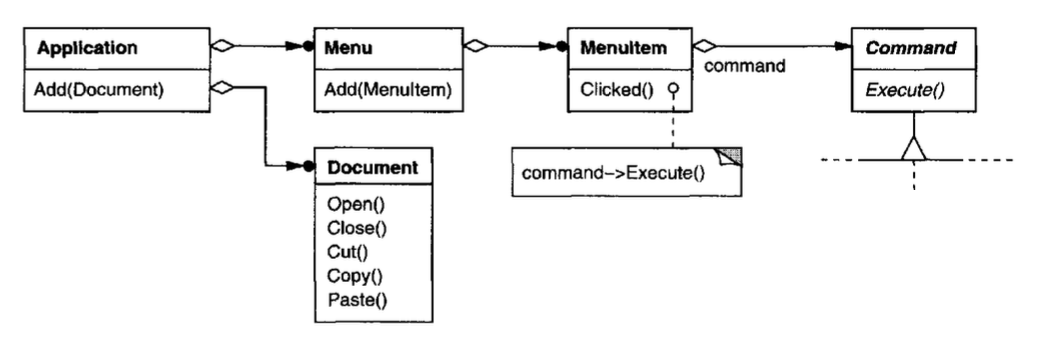
\includegraphics[width=1\linewidth]{assets/pattern/command/command-esempio-1.png}
    \end{figure}
    \begin{figure}[H]
        \centering
        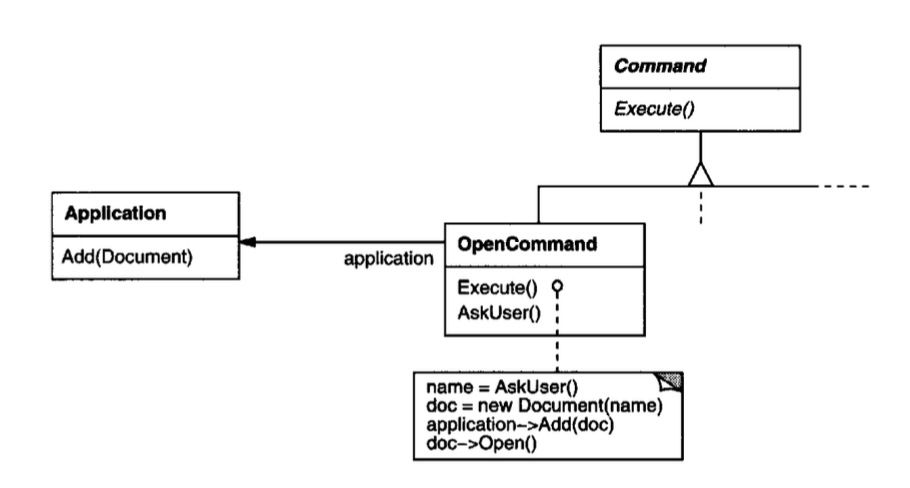
\includegraphics[width=1\linewidth]{assets/pattern/command/command-esempio-3.png}
    \end{figure}
    \columnbreak
    \begin{figure}[H]
        \centering
        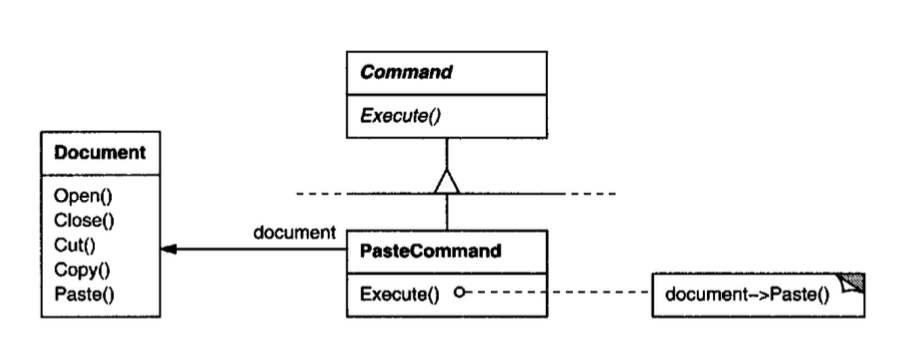
\includegraphics[width=1\linewidth]{assets/pattern/command/command-esempio-2.png}
    \end{figure}
    \begin{figure}[H]
        \centering
        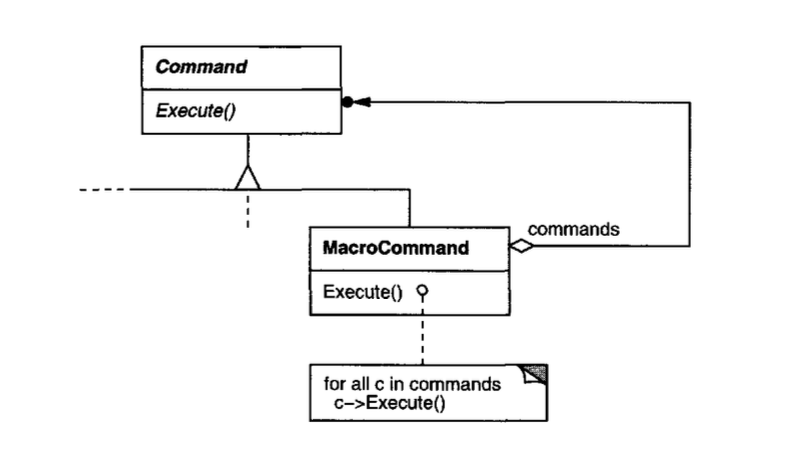
\includegraphics[width=1\linewidth]{assets/pattern/command/command-esempio-4.png}
    \end{figure}
\end{multicols}

Il pattern Command permette agli oggetti del toolkit di fare richieste ad oggetti applicativi non specificati trasformando la richiesta stessa in un oggetto che può essere memorizzato e passato come altri oggetti. La chiave di questo pattern è una classe astratta Command che dichiara un'interfaccia per eseguire operazioni, nella forma più semplice includendo un'operazione astratta Execute. Le sottoclassi concrete Command specificano una coppia destinatario-azione memorizzando il destinatario come variabile di istanza e implementando Execute per invocare la richiesta, dove il destinatario ha la conoscenza necessaria per eseguire la richiesta. I menu possono essere implementati facilmente con oggetti Command: ogni scelta in un menu è un'istanza della classe MenuItem, e quando l'utente seleziona un MenuItem, questo chiama Execute sul suo comando. I MenuItem non sanno quale sottoclasse di Command usano, mentre le sottoclassi Command memorizzano il destinatario della richiesta e invocano una o più operazioni su di esso. Notate come in tutti questi esempi il pattern Command disaccoppi l'oggetto che invoca l'operazione da quello che ha la conoscenza per eseguirla, dandoci grande flessibilità nella progettazione dell'interfaccia utente e permettendoci di sostituire comandi dinamicamente, supportare scripting di comandi componendo comandi in altri più grandi, tutto questo perché l'oggetto che emette una richiesta deve solo sapere come emetterla, non come verrà eseguita.

\paragraph{Applicabilità} È consigliabile utilizzare il pattern Command quando:
\begin{itemize}
    \item Si vogliono parametrizzare oggetti in base ad un'azione da eseguire;
    \item Si vogliono specificare, mettere in coda ed eseguire richieste in momenti diversi;
    \item Si vuole supportarte l'\textit{undo} delle operazioni;
    \item Si vogliono memorizzare le modifiche in modo che possano essere riapplicate in caso di crash del sistema;
    \item Si vuole strutturare un sistema attorno ad operazioni di alto livello basate su operazioni primitive,
\end{itemize}

\begin{figure}[H]
    \centering
    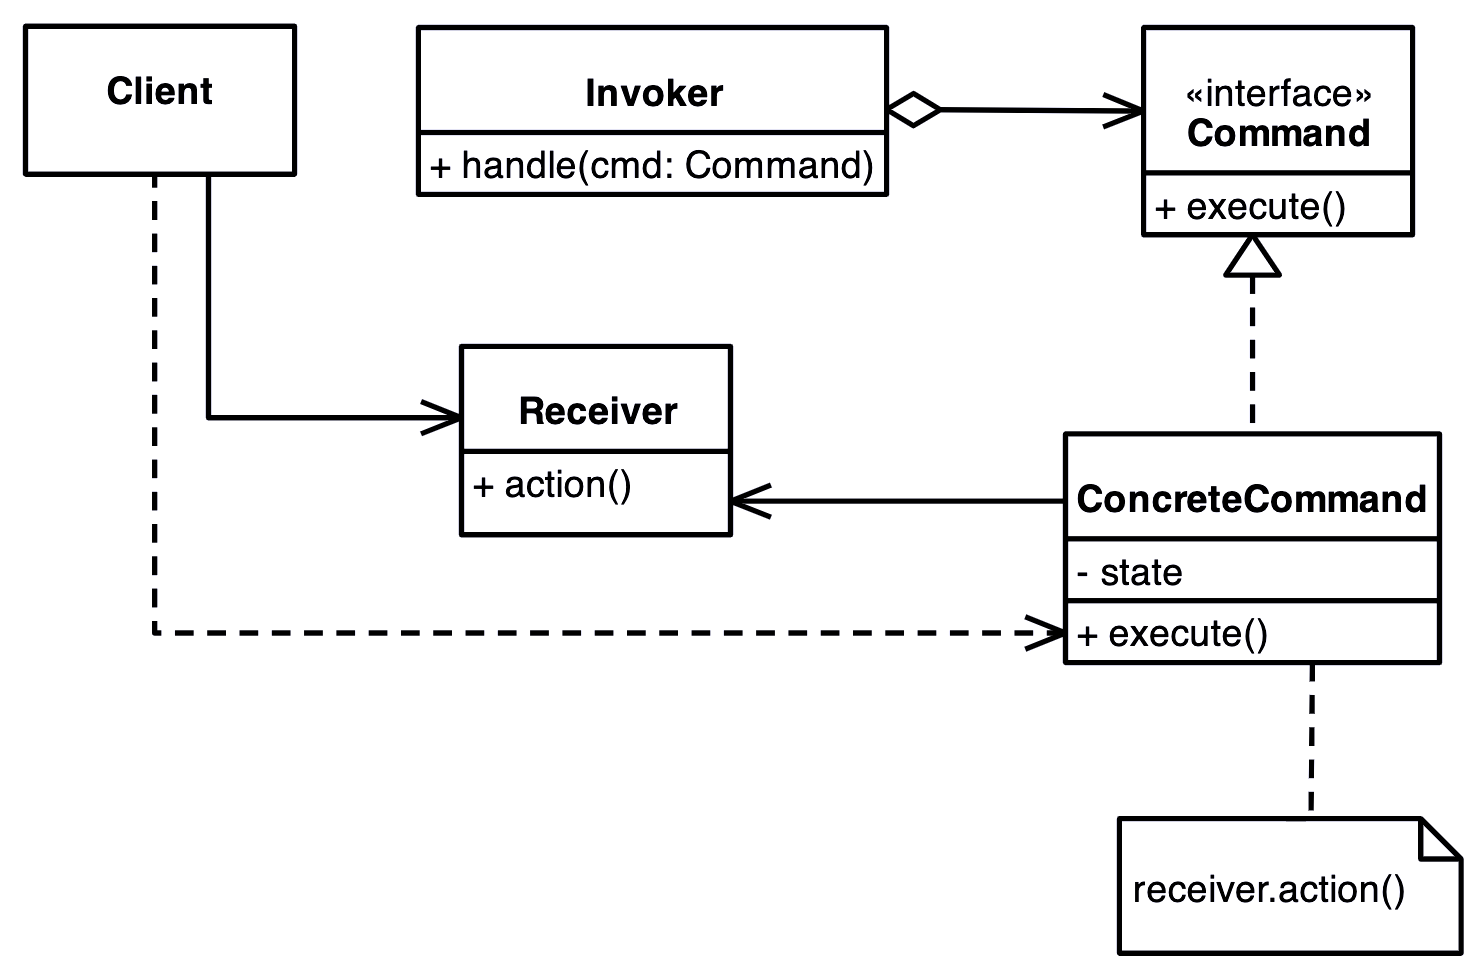
\includegraphics[width=0.75\linewidth]{assets/pattern/command/command-struttura.png}
    \caption{Class Diagram del pattern Command}
\end{figure}

\paragraph{Struttura} Il pattern Command è composto da:
\begin{itemize}
    \item \textbf{Command}: dichiara un’interfaccia per l’esecuzione di un’operazione generica.
    \item \textbf{ConcreteCommand} (PasteCommand, OpenCommand): definisce un legame fra un oggetto destinatario e un’azione. Implementa il metodo execute() invocando il metodo (i metodi) corrispondente sul Receiver.
    \item \textbf{Client} (Application): crea un’istanza concreta di Command e ne imposta il Receiver.
    \item \textbf{Invoker} (MenuItem): chiede a Command di portare a termine la richiesta
    \item \textbf{Receiver} (Document, Application): conosce il modo di svolgere le operazioni associate a una richiesta. Qualsiasi classe può essere vista come Receiver.
\end{itemize}

Il Client crea un oggetto ConcreteCommand e specifica chi lo riceve. L'Invoker salva il ConcreteCommand e effettua una richiesta chiamando la \textit{Execute()} sul Command (se l'\textit{undo()} è supportato il ConcreteCommand salva lo stato). Il ConcreteCommand invoca l'operazione e il suo ricettore la esegue.

\begin{figure}[H]
    \centering
    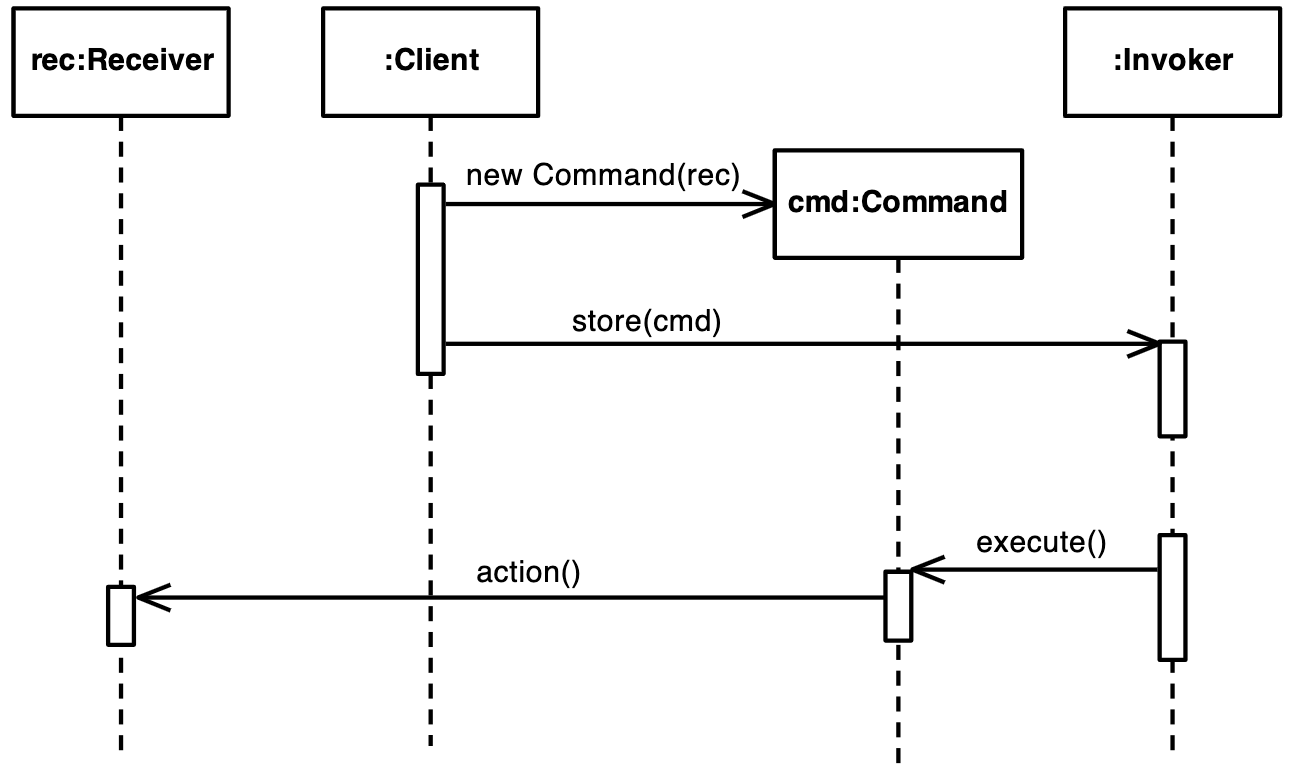
\includegraphics[width=0.75\linewidth]{assets/pattern/command/command-sequence.png}
    \caption{Sequence Diagram del pattern Command}
\end{figure}

\paragraph{Conseguenze} Command disaccoppia l’oggetto che invoca un’operazione da quello che conosce come portarla a termine.
Gli oggetti Command sono oggetti a tutti gli effetti, possono essere manipolati ed estesi con un qualsiasi altro oggetto.
È possibile comporre più comandi in un comando composito.
In generale, i comandi compositi sono un’istanza del pattern Composite.
Risulta facile aggiungere nuovi comandi poiché non è necessario modificare le classi esistenti


\newpage